\documentclass{article}

% Geometry package
\usepackage[a4paper, margin=1in]{geometry}
\usepackage{multicol}

% Math packages
\usepackage{amsmath}
\usepackage{amssymb}
\usepackage{amsthm}

% Other packages
\usepackage{hyperref}
\usepackage{float}

% Captions
\usepackage{caption}
\usepackage{subcaption}

% Graphics
\usepackage{graphicx}
\usepackage{tikz}
\usepackage{forest}

% Bibliography
\usepackage[style=ieee, backend=biber]{biblatex}
\addbibresource{ref.bib}

% Code
\usepackage{listings}
\usepackage{xcolor}
 
% Code style
\lstdefinestyle{Python}{
   language=Python,
    basicstyle=\ttfamily\footnotesize,
    keywordstyle=\color{blue},
    commentstyle=\color{orange},
    stringstyle=\color{red},
    showstringspaces=false,
    breaklines=true,
    breakatwhitespace=true,
    tabsize=2,
    numbers=left,
    numberstyle=\tiny,
    numbersep=5pt,
    frame=single,
    framesep=5pt,
    xleftmargin=15pt,
    xrightmargin=15pt,
    aboveskip=0pt,
    belowskip=0pt,
    backgroundcolor=\color{white}
  }

\renewcommand{\maketitle}{
  \begin{flushleft}
    ZC - University of Science and Technology
    \hfill Fall 2023 \\
    MATH 201: Linear Algebra and Vector Geometry
  \end{flushleft}
  \begin{center}
    \Huge Equilibrium Temperature Distributions \\
    \LARGE \textit{Using Linear Algebra}
  \end{center}
  \begin{flushleft}
    Team Members: \\

    \begin{tabular}{ccc}
      202200102 & Ali Ehab & \href{mailto:s-ali.aziz@zewailcity.edu.eg}{s-ali.aziz@zewailcity.edu.eg} \\
      202200776 & Marwan Basem & \href{mailto:s-marwan.hussien@zewailcity.edu.eg}{s-marwan.hussien@zewailcity.edu.eg} \\
      202201079 & SalahDin Rezk & \href{mailto:s-salahdin.rezk@zewailcity.edu.eg}{s-salahdin.rezk@zewailcity.edu.eg} \\
    \end{tabular}  \\
  \end{flushleft}
}

\begin{document}

\maketitle
\tableofcontents
\listoffigures

\begin{abstract}
The study of the heat equation has been instrumental in thermodynamics; we consider one of the most famous sets of problems in Differential Equations, the Dirichlet Boundary value problem~\cite{stein}. We study the temperature inside a plate which is in thermal equilibrium for which we only know the temperature on the boundary. We are providing numerical solutions utilizing many of the tools developed in Linear Algebra.    
\end{abstract}

\begin{multicols}{2}
  
\section{Introduction}
The heat equation is a fundamental partial differential equation that describes the distribution of heat in a system over time and space. It is given by:

\begin{equation}
  \frac{\partial u}{\partial t} = \Delta u
\end{equation}

where $u$ represents the temperature distribution, $t$ is time, and $\Delta$ is the Laplacian operator. This equation is widely used in various fields, including physics, engineering, and mathematics, to model heat transfer phenomena.

In this context, we are interested in studying systems that reach thermal equilibrium, where the temperature distribution remains constant over time ($\frac{\partial u}{\partial t} = 0$). This special case of the heat equation can be written as:

\begin{equation}
  \Delta u = 0
\end{equation}

This equation is known as the steady-state heat equation or Laplace's equation. It describes the temperature distribution in a system that has reached a state of balance, where the heat flow is constant and there are no sources or sinks of heat.

Solutions to Laplace's equation possess a remarkable property known as the mean-value property. This property states that if $u$ is a solution to $\Delta u = 0$, then the value of $u$ at any point $(x,y)$ is equal to the average of its values on a circle centered at $(x,y)$. Mathematically, this can be expressed as:

\begin{equation}
  u(x,y) = \frac{1}{2\pi} \int_{0}^{2\pi}u(x + r \: \cos\,\theta, y + r \: \sin\,\theta) d\theta
\end{equation}

where $r$ represents the radius of the circle and $\theta$ is the angle of rotation.

This mean-value property provides valuable insights into the behavior of solutions to Laplace's equation and has important implications in various areas of mathematics and physics. It allows us to understand the relationship between the values of a function at different points and provides a powerful tool for solving problems involving Laplace's equation. \cite{anton}

\section{Problem}
In this problem, we are given the temperature distribution on the boundaries of a plate that is in thermal equilibrium. Our goal is to determine the temperature distribution inside the plate based solely on the boundary conditions. We need to solve the steady-state heat equation, $\Delta u = 0$, numerically to obtain the desired solution.

\section{Solution}
To solve the steady-state heat equation numerically, we start by creating an $n\times n$ grid, where the lattice points represent the locations at which we will compute the temperature. This grid allows us to discretize the problem and approximate the continuous temperature distribution.

Since we are dealing with Laplace's equation, we can apply the mean-value property to our discrete setup. This property states that the temperature at any point on the grid is equal to the average of the temperatures of its neighboring points. Mathematically, this can be expressed as:

\begin{equation}
  T_{i, j} = \frac{1}{4} ( T_{i+1,j} + T_{i-1,j} + T_{i,j+1} + T_{i,j-1})
\end{equation}

where $T_{i, j}$ represents the temperature at the point $(i,j)$ on the grid.

\begin{figure}[H]
  \begin{center}
    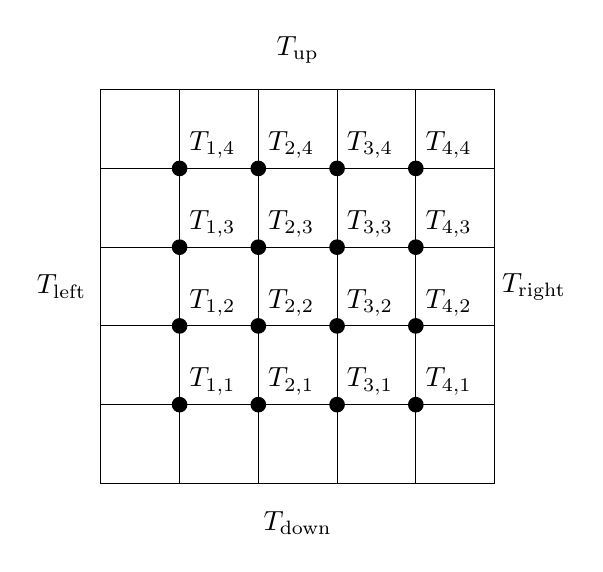
\begin{tikzpicture}
      % Define the size of the square and the number of grid points
      \def\squaresize{5}
      \def\gridsize{5}
      % Draw the square
      \draw (0,0) rectangle (\squaresize, \squaresize);
      % Draw the grid
      \foreach \x in {0,...,\gridsize} {
        \draw (\x*\squaresize/\gridsize, 0) -- (\x*\squaresize/\gridsize, \squaresize);
        \draw (0, \x*\squaresize/\gridsize) -- (\squaresize, \x*\squaresize/\gridsize);
      }
      % Label each point as T_i,j
      \foreach \i in {1,...,4}{
        \foreach \j in {1,...,4}{
          \draw (\i/\gridsize*\squaresize, \j/\gridsize*\squaresize) node[circle, fill, inner sep=2pt]{} node[above right] {$T_{\i,\j}$};
        }
      }
      % Boundary conditions
      \draw (-0.5, 2.5) node {$T_{\text{left}}$};
      \draw (2.5, 5.5) node {$T_{\text{up}}$};
      \draw (5.5, 2.5) node {$T_{\text{right}}$};
      \draw (2.5, -0.5) node {$T_{\text{down}}$};
    \end{tikzpicture}
  \end{center}
  \caption{Example of a $n=4$ square grid}
\end{figure}


By applying this equation to every point on the grid, we obtain a system of linear equations. This system can be written in matrix form as:

\begin{equation}
  \textbf{t} = M \textbf{t} + \textbf{b}
\end{equation}

where $\textbf{t}$ is a column vector representing the unknown temperatures, $M$ is the matrix containing the coefficients of the unknown temperatures, and $\textbf{b}$ is a column vector that represents the right-hand side of the system.

We can solve this system using two different methods: the inverse matrix method and the Jacobi iteration method.

\subsection{Inverse Matrix Method}
In the inverse matrix method, we rewrite the equation as:

\begin{align}
  \textbf{t} &= M \textbf{t} + \textbf{b} \\
  (\textbf{\textit{I}} - M)\textbf{t} &= \textbf{b} \\
  \textbf{t} &= (\textbf{\textit{I}} - M)^{-1} \textbf{b}
\end{align}

where $\textbf{\textit{I}}$ is the identity matrix.

By computing the inverse of the matrix $(\textbf{\textit{I}} - M)$, we can obtain the solution vector $\textbf{t}$, which represents the temperature distribution inside the plate.

\subsection{Jacobi Iteration Method}
The Jacobi iteration method is an iterative technique that allows us to approximate the solution to the system of linear equations. It involves repeatedly updating the temperature values at each point on the grid until convergence is achieved.

The Jacobi iteration formula for our problem can be written as:

\begin{equation}
  T_{i, j}^{(k+1)} = \frac{1}{4} ( T_{i+1,j}^{(k)} + T_{i-1,j}^{(k)} + T_{i,j+1}^{(k)} + T_{i,j-1}^{(k)})
\end{equation}

where $T_{i, j}^{(k)}$ represents the temperature at point $(i,j)$ in the $k$-th iteration.

We start with an initial guess for the temperature distribution and update the values at each point using the Jacobi iteration formula. We continue this process until the temperature values converge to a stable solution.

Both the inverse matrix method and the Jacobi iteration method provide solutions to the steady-state heat equation. The choice of method depends on the specific requirements of the problem and the desired accuracy of the solution.

By implementing these methods and solving the system of linear equations, we can determine the temperature distribution inside the plate based on the given boundary conditions. This allows us to gain insights into the heat transfer behavior and study the thermal equilibrium of the system.

\section{Implementation}
The code was heavily inspired by \cite{gandhi, matlab}. The project was
implemented using \href{https://www.python.org/}{Python 3.12.0} and
\href{https://python-poetry.org/}{Poetry 1.6.1} for package and tendency
management. The reason behind choosing Python is that it is a high-level
language that is easy to read and write. It also has a lot of libraries that
make it easy to implement the project. In addition, Poetry provides a friendly
and dynamic interface for interacting with the complex system of python
libraries while ensuring consistency.

Furthermore, \href{https://git-scm.com/}{Git 2.43.0} was used for version
control and \href{github.com}{GitHub} for hosting the code repository. Git
provided a simple and efficient way to track changes and collaborate on the
project, while GitHub allowed us to share our code and work together on the
project remotely. Both of these tools were essential in the development process
and contributed significantly to the success of the project.

\subsection{Code Structure}
The code is structured into different modules, each of which contains a set of
functions that perform a specific task. This modular approach allows us to
organize the code and make it easier to maintain. Directory structure is shown
below.
\end{multicols}

\begin{figure}[H]
  \begin{forest}
    for tree={
      font=\ttfamily,
      grow'=0,
      child anchor=west,
      parent anchor=south,
      anchor=west,
      calign=first,
      edge path={
        \noexpand\path [draw, \forestoption{edge}]
        (!u.south west) +(7.5pt,0) |- node[fill,inner sep=1.25pt] {} (.child anchor)\forestoption{edge label};
      },
      before typesetting nodes={
        if n=1
        {insert before={[,phantom]}}
        {}
      },
      fit=band,
      before computing xy={l=15pt},
    }
    [ETD-LA
    [poetry.lock]
    [pyproject.toml]
    [src
    [etd\_la
    [\_\_init\_\_.py]
    [main.py]
    [matrix\_solvers.py]
    [plotting.py]
    [temperature\_solver.py]
    ]
    ]
    ]
  \end{forest}
  \caption{Project Hierarchy}
\end{figure}

\begin{multicols}{2}
\subsection{Importing libraries}
We start by importing the necessary libraries for our implementation. We will be
using the \texttt{numpy} library for linear algebra operations and the
\texttt{matplotlib} library for plotting. We also import the
\texttt{Axes3D} class from the \texttt{mpl\_toolkits.mplot3d} module to enable
3D plotting. 
\end{multicols}

\begin{lstlisting}[style=Python]
import numpy as np
import matplotlib.pyplot as plt
from mpl_toolkits.mplot3d import Axes3D
\end{lstlisting}

\begin{multicols}{2}
\subsection{Solver functions}
\subsubsection{Inverse matrix}
We can compute the inverse of $\textbf{\textit{I}} - M$ using the following
python code. This function takes the coefficient matrix $M$ and the right-hand
side vector $b$ as inputs, then calculates the inverse of $M$ and multiplies it
by $b$ to obtain the solution vector $x$. The efficiency of this method is to be
tested in the appendix.
\end{multicols}
\begin{lstlisting}[style=Python]
def calculate_inverse_solution(A, b):
    A_inverse = np.linalg.inv(A)
    x = np.dot(A_inverse, b)
    return x
\end{lstlisting}

\begin{multicols}{2}
\subsubsection{Jacobi iterations}
We start with an initial guess for $\textbf{t}_0$, and we iteratively plug it in the equation
\begin{equation}
  \textbf{t}_n = M \textbf{t}_n-1 + b
\end{equation}
each value $\textbf{t}_n$ is a better approximation for the exact solution.
The following Python code implements the Jacobi iteration method. It takes the
coefficient matrix $M$, the right-hand side vector $b$, an initial guess $x_0$,
a tolerance value \texttt{tol}, and a maximum number of iterations \texttt{max\_iter} as
inputs. It then iteratively updates the temperature values at each point on the
grid until convergence is achieved. If the solution does not converge within the
specified number of iterations, an error is raised. This is done to prevent the
program from running indefinitely in case the solution does not converge.
\end{multicols}

\begin{lstlisting}[style=Python]
def jacobi_iteration(A, b, x0=None, tol=1e-6, max_iter=1000):
    n = len(b)
    x = x0 if x0 is not None else np.zeros(n)
    z_iter = np.zeros((max_iter, n))

    for k in range(max_iter):
        x_new = np.zeros_like(x)

        for i in range(n):
            sigma = np.dot(A[i, :i], x[:i]) + np.dot(A[i, i + 1 :], x[i + 1 :])
            x_new[i] = (b[i] - sigma) / A[i, i]
            z_iter[k] = x_new

        if np.linalg.norm(x_new - x) < tol:
            return x_new, k + 1, z_iter[:k + 1]

        x = x_new

    raise ValueError(
        "Jacobi iteration did not converge within the specified number of iterations."
    )
\end{lstlisting}

\begin{multicols}{2}
\subsection{Solving the system}
\subsubsection{Creating the coefficient matrix}
We start by creating the coefficient matrix $M$.
We can do this by creating a matrix of zeros, and then filling it with the
coefficients of the unknown temperatures. The following Python code implements
this approach. It takes the size of the grid $n$ and the boundary temperatures
as inputs and returns the coefficient matrix $M$ and the right-hand side vector
$b$. The boundary temperatures are specified as follows: \texttt{left\_temp} for
the left boundary, \texttt{up\_temp} for the upper boundary, \texttt{right\_temp}
for the right boundary, and \texttt{down\_temp} for the lower boundary.
\end{multicols}

\begin{lstlisting}[style=Python]
def generate_coefficient_matrix(size, left_temp, up_temp, right_temp, down_temp):
    matrix = np.zeros((size * size, size * size))
    rhs_vector = np.zeros(size * size)

    for row in range(size):
        for col in range(size):
            point_num = size * row + col
            if col - 1 >= 0:
                matrix[point_num][point_num - 1] = 1
            else:
                rhs_vector[point_num] += left_temp

            if row - 1 >= 0:
                matrix[point_num][point_num - size] = 1
            else:
                rhs_vector[point_num] += up_temp

            if col + 1 < size:
                matrix[point_num][point_num + 1] = 1
            else:
                rhs_vector[point_num] += right_temp

            if row + 1 < size:
                matrix[point_num][point_num + size] = 1
            else:
                rhs_vector[point_num] += down_temp

    return matrix, rhs_vector
\end{lstlisting}

\begin{multicols}{2}
\subsubsection{Temperature Equation}
Now that we have the coefficient matrix $M$ and the right-hand side vector $b$,
we can solve the temperature equation. The following Python code implements this
approach. It takes the size of the grid $n$ and the boundary temperatures as
inputs and returns the solution vector $x$. The multiplication by 4 is done to
account for the \(\frac{1}{4}\) coefficient in the mean-value property while the
\texttt{np.identity} is done to account for the \textbf{\textit{I}} matrix in
the equation. The \texttt{solve\_temperature\_equation} function is a wrapper
function that combines the steps of generating the coefficient matrix and
solving the temperature equation. The \texttt{calculate\_inverse\_solution}
function is used by default.
\end{multicols}

\begin{lstlisting}[style=Python]
def solve_temperature_equation(size, left_temp, up_temp, right_temp, down_temp):
    coefficient_matrix, rhs_vector = generate_coefficient_matrix(
        size, left_temp, up_temp, right_temp, down_temp
    )

    # Uncomment one of the following lines based on your preferred solver
    # temperature_solution, _ = jacobi_iteration(4 * np.identity(size * size) - coefficient_matrix, rhs_vector)
    temperature_solution = calculate_inverse_solution(
        4 * np.identity(size * size) - coefficient_matrix, rhs_vector
    )

    return temperature_solution
\end{lstlisting}

\begin{multicols}{2}
\subsection{Plotting}
To visualize the equilibrium temperature distribution on the plate, we can
create a heat map plot with contour lines representing isothermal lines. The
following Python code implements this approach. It takes the size of the grid
$n$ and the solution vector $x$ as inputs and plots the temperature distribution
on the plate. The \texttt{plot\_temperature\_distribution\_2d} function is used
to plot the temperature distribution on a 2D grid, while the
\texttt{plot\_temperature\_distribution\_3d} function is used to plot the
temperature distribution on a 3D grid. In both cases, the \texttt{cmap}
parameter is used to specify the color map, while the \texttt{interpolation}
parameter is used to specify the interpolation method to smooth the image.
\end{multicols}

\subsubsection{2D Plot}
\begin{lstlisting}[style=Python]
def plot_temperature_distribution_2d(size, temperature):
    plt.imshow(
        temperature.reshape(size, size), cmap="RdYlBu_r", interpolation="gaussian"
    )
    plt.colorbar()
    plt.contour(temperature.reshape(size, size), cmap="hot")
    plt.title("Temperature Distribution")
    plt.xlabel("Column Index")
    plt.ylabel("Row Index")
    plt.show()

# Plot the temperature distribution
plot_temperature_distribution_2d(n, x)
\end{lstlisting}

\subsubsection{3D Plot}
\begin{lstlisting}[style=Python]
def plot_temperature_distribution_3d(size, temperature):
    fig = plt.figure()
    ax = fig.add_subplot(111, projection="3d")
    x = np.arange(0, size, 1)
    y = np.arange(0, size, 1)
    X, Y = np.meshgrid(x, y)
    ax.plot_surface(X, Y, temperature.reshape(size, size), cmap="RdYlBu_r", alpha=0.75)
    ax.contour(X, Y, temperature.reshape(size, size), cmap="hot")
    ax.set_title("Temperature Distribution")
    ax.set_xlabel("Column Index")
    ax.set_ylabel("Row Index")
    ax.set_zlabel("Temperature")
    plt.show()
\end{lstlisting}

\begin{multicols}{2}
\section{Results}
We tested our implementation on a variety of boundary conditions to gain
insights into the behavior of the temperature distribution. The results obtained
through this process are presented below. Both 2D and 3D plots are included to
visualize the temperature distribution on the plate. The color map used in the
plots is \texttt{RdYlBu\_r}, while the interpolation method is \texttt{gaussian}
for the 2D plots and \texttt{linear} for the 3D plots. We can observe that the
temperature distribution is symmetric about the center of the plate, which is
consistent with the mean-value property of solutions to Laplace's equation.
However, the last case is an edge case where the temperature distribution is not
symmetric due to the boundary conditions.
\end{multicols}

\begin{figure}[H]
  \begin{subfigure}{0.45\textwidth}
    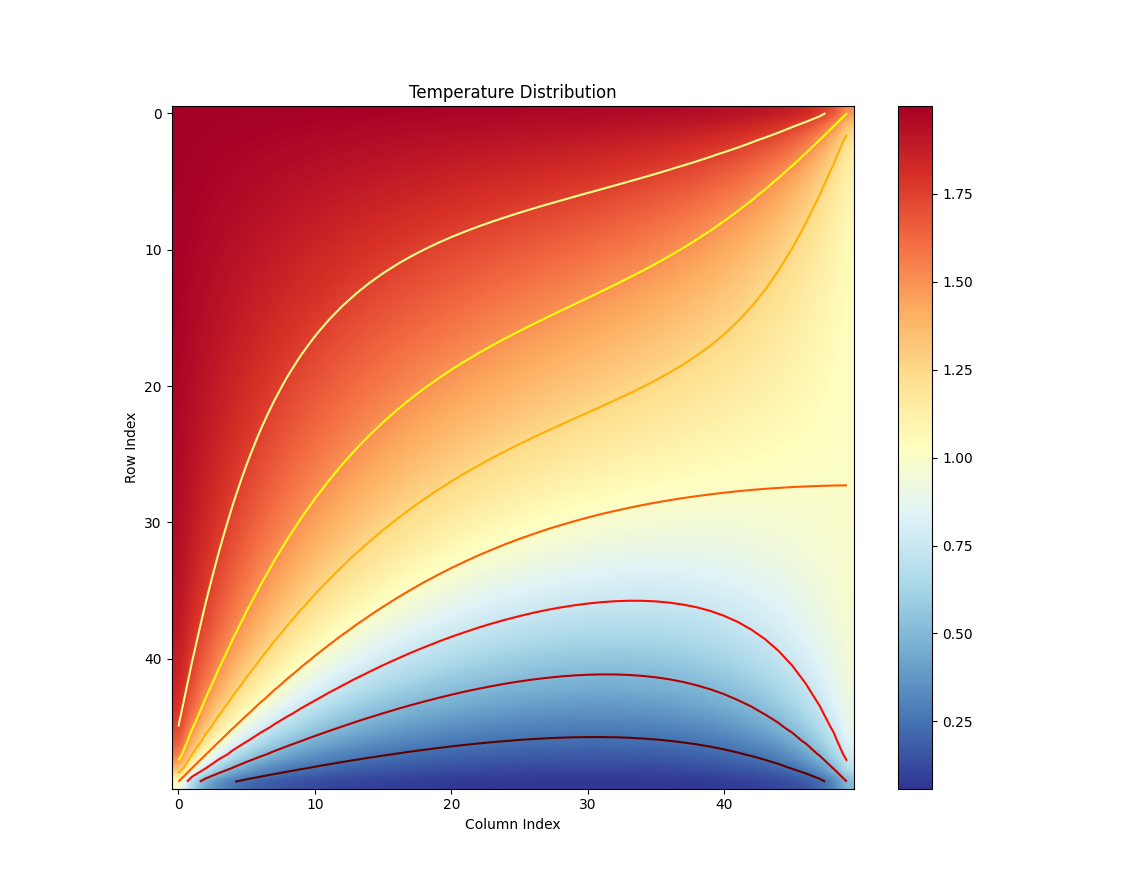
\includegraphics[width=\linewidth]{figures/Figure_1.png}
    \caption{2D Plot}
  \end{subfigure}
  \hfill
  \begin{subfigure}{0.45\textwidth}
    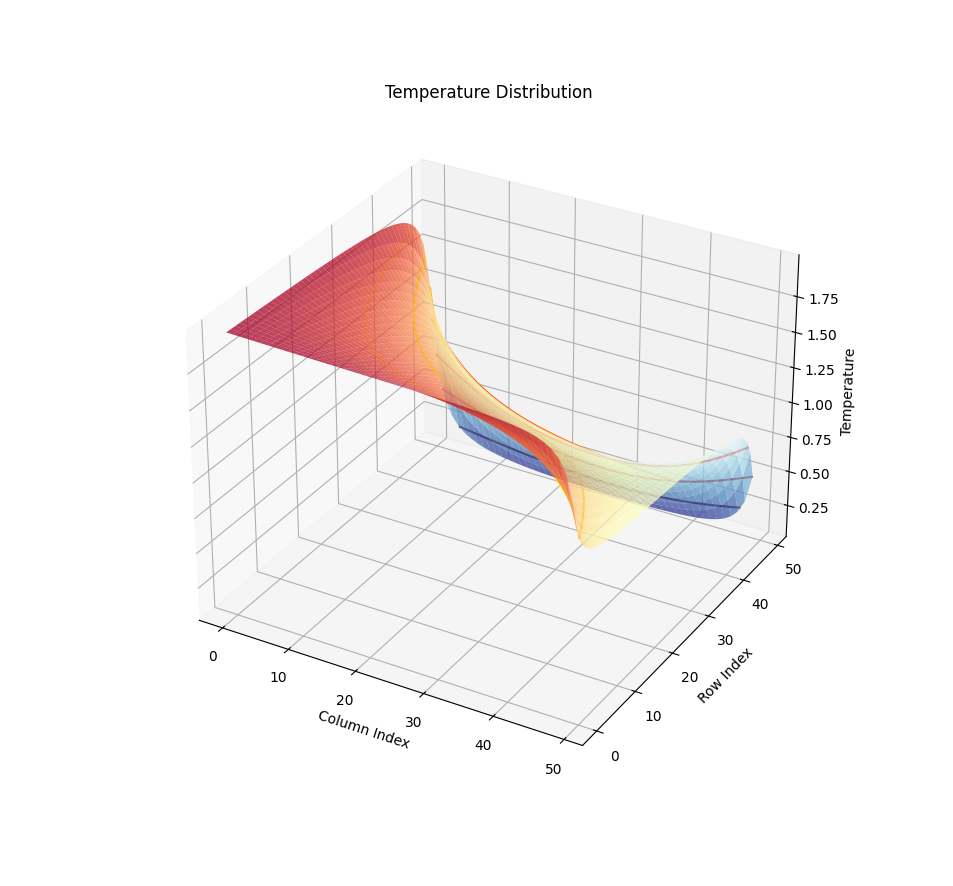
\includegraphics[width=\linewidth]{figures/Figure_2.png}
    \caption{3D Plot}
  \end{subfigure}
  \caption{Boundaries $T_{\text{left}}=2, T_{\text{up}}=2, T_{\text{right}}=1, T_{\text{down}}=0$}
\end{figure}

\begin{figure}[H]
  \begin{subfigure}{0.45\textwidth}
    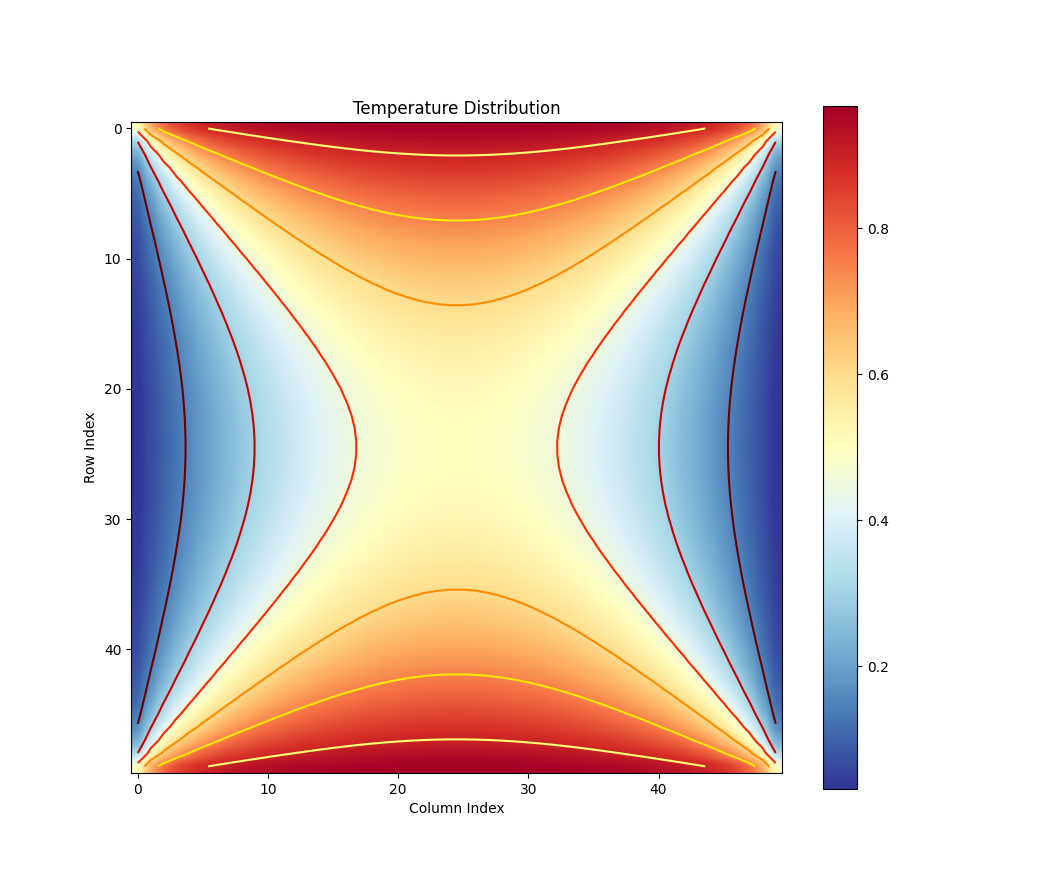
\includegraphics[width=\linewidth]{figures/Figure_3.png}
    \caption{2D Plot}
  \end{subfigure}
  \hfill
  \begin{subfigure}{0.45\textwidth}
    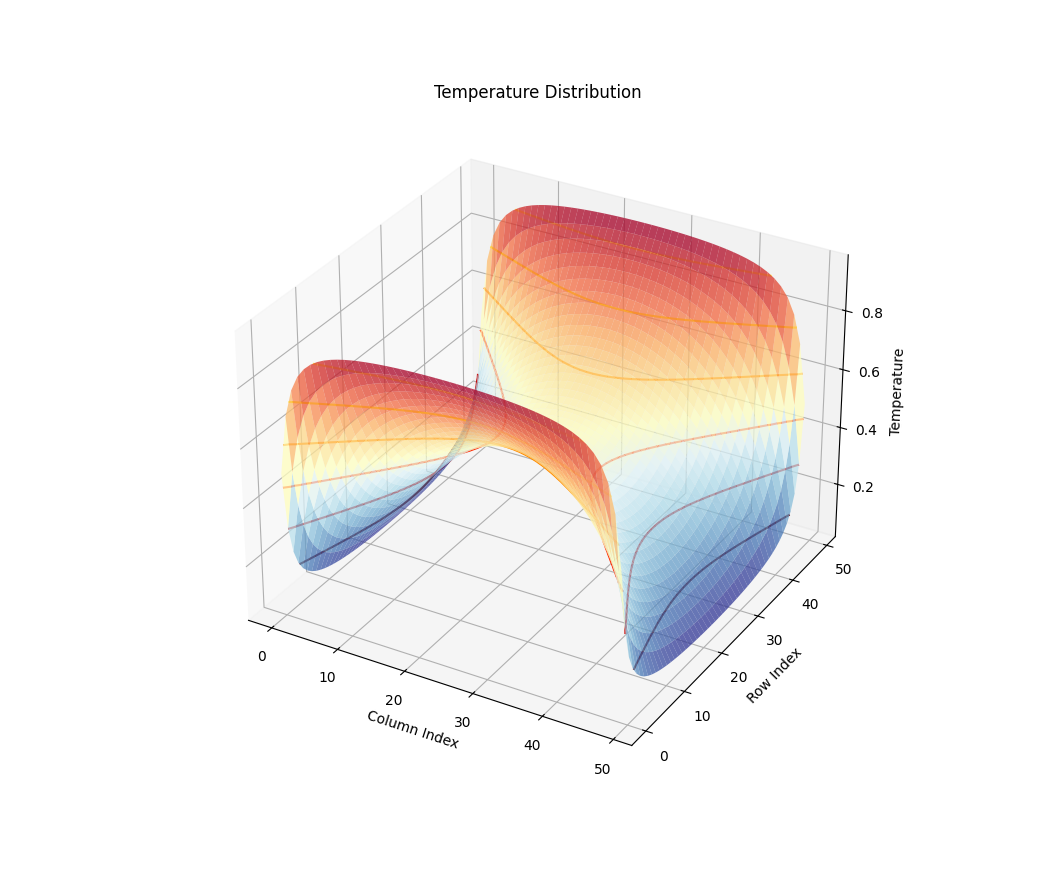
\includegraphics[width=\linewidth]{figures/Figure_4.png}
    \caption{3D Plot}
  \end{subfigure}
  \caption{Boundaries $T_{\text{left}}=0, T_{\text{up}}=1, T_{\text{right}}=0, T_{\text{down}}=1$}
\end{figure}

\begin{figure}[H]
  \begin{subfigure}{0.45\textwidth}
    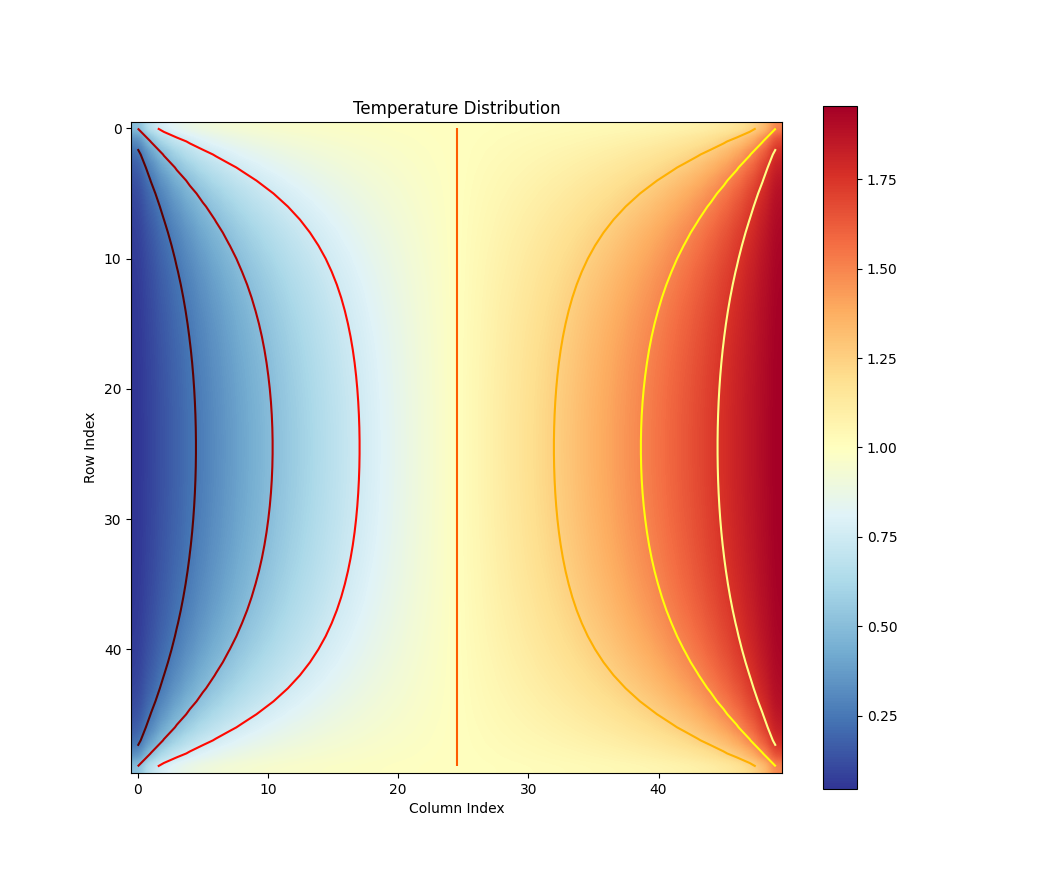
\includegraphics[width=\linewidth]{figures/Figure_5.png}
    \caption{2D Plot}
  \end{subfigure}
  \hfill
  \begin{subfigure}{0.45\textwidth}
    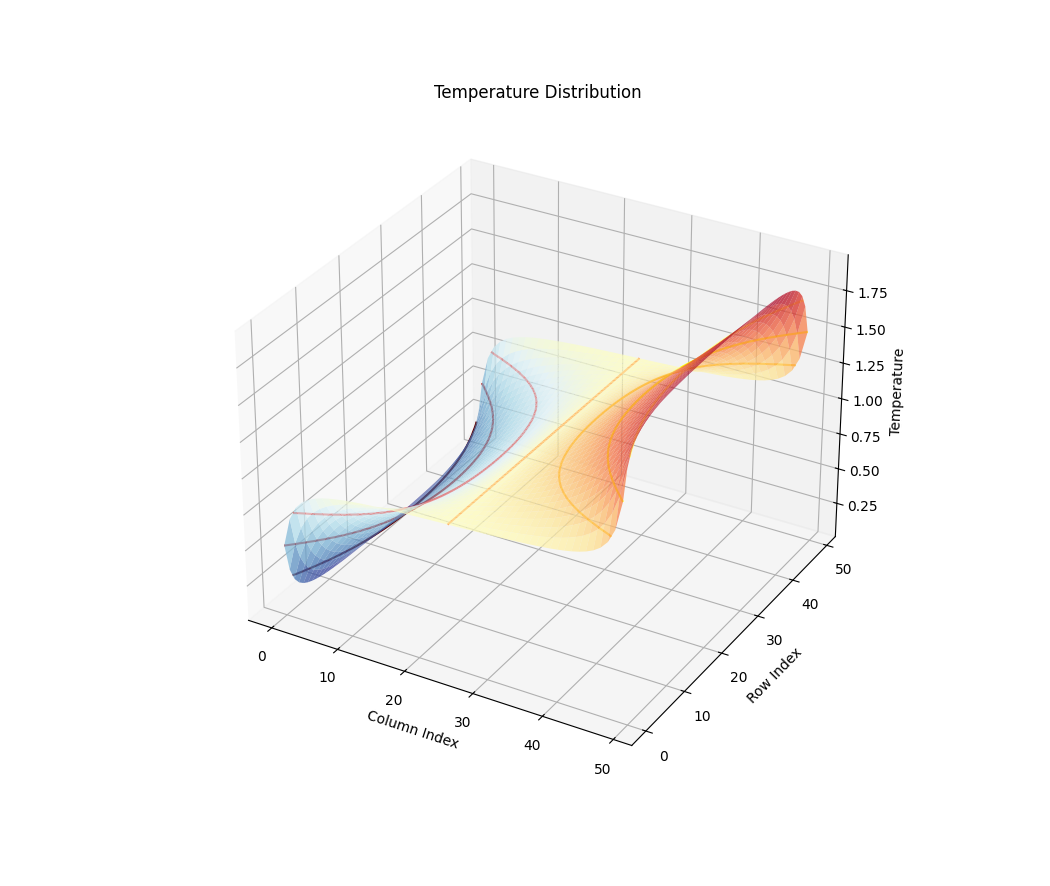
\includegraphics[width=\linewidth]{figures/Figure_6.png}
    \caption{3D Plot}
  \end{subfigure}
  \caption{Boundaries $T_{\text{left}}=0, T_{\text{up}}=1, T_{\text{right}}=2, T_{\text{down}}=1$}
\end{figure}

\begin{figure}[H]
  \begin{subfigure}{0.45\textwidth}
    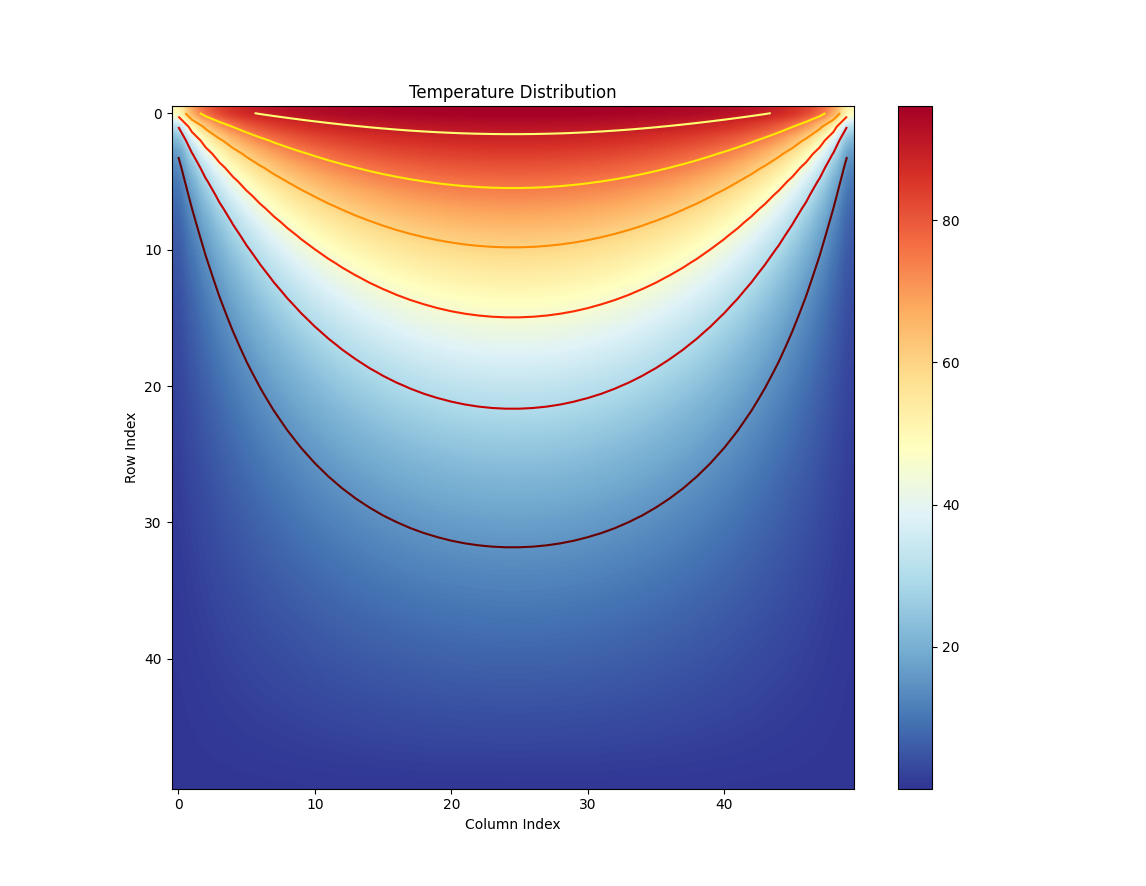
\includegraphics[width=\linewidth]{figures/Figure_9.png}
    \caption{2D Plot}
  \end{subfigure}
  \hfill
  \begin{subfigure}{0.45\textwidth}
    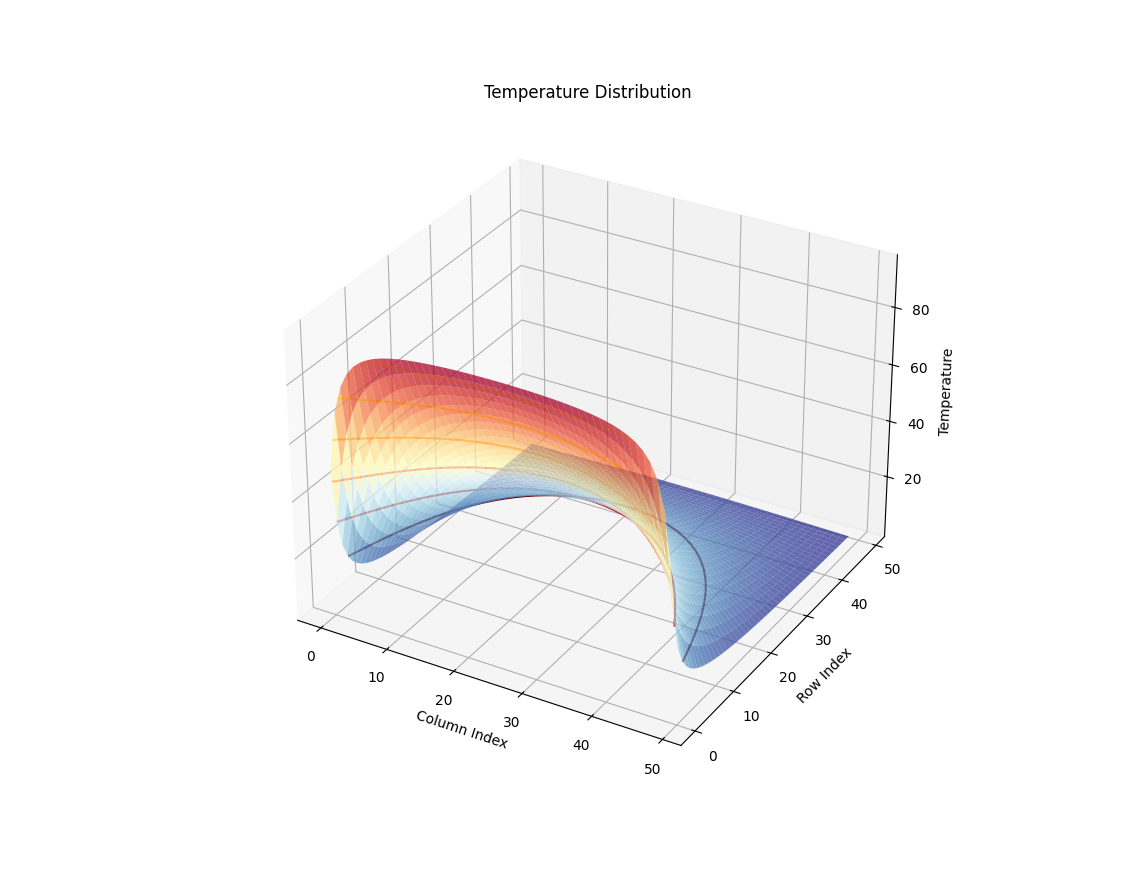
\includegraphics[width=\linewidth]{figures/Figure_10.png}
    \caption{3D Plot}
  \end{subfigure}
  \caption{Boundaries $T_{\text{left}}=0, T_{\text{up}}=100, T_{\text{right}}=0, T_{\text{down}}=0$}
\end{figure}

\begin{figure}[H]
  \begin{subfigure}{0.45\textwidth}
    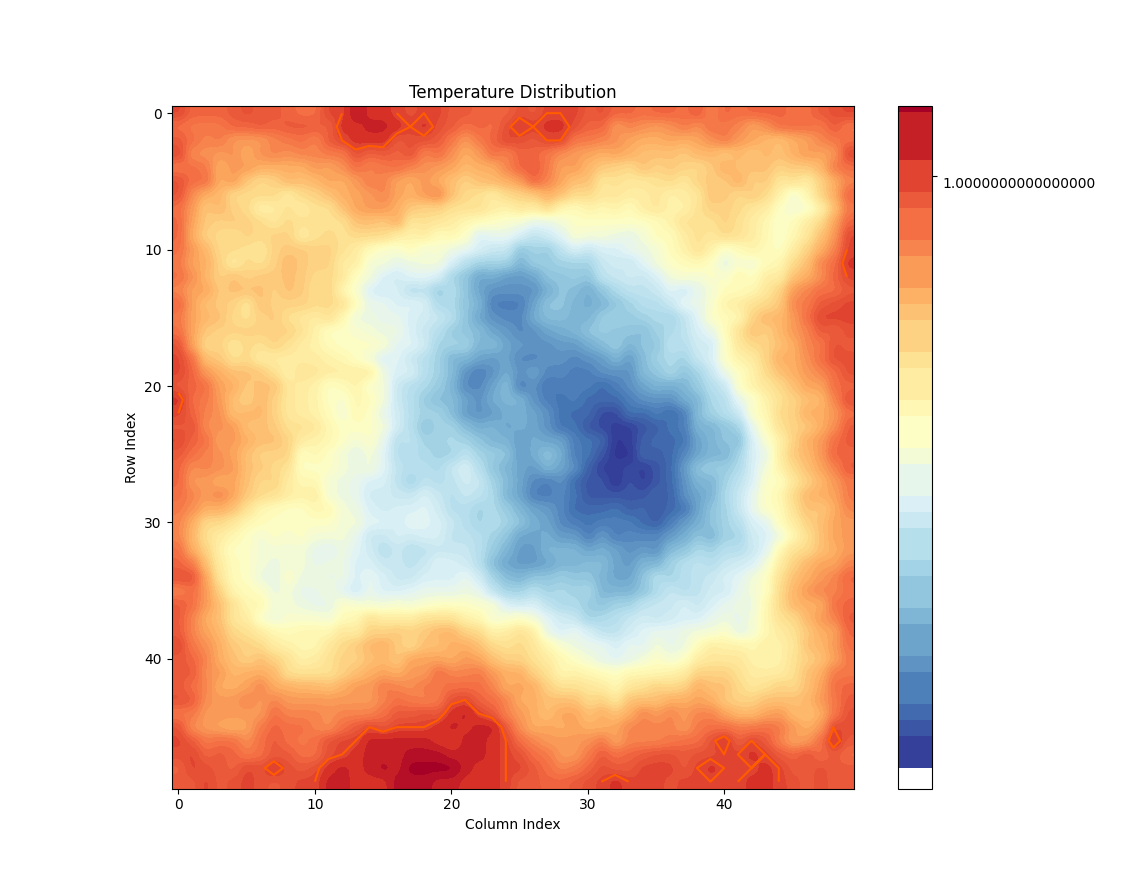
\includegraphics[width=\linewidth]{figures/Figure_7.png}
    \caption{2D Plot}
  \end{subfigure}
  \hfill
  \begin{subfigure}{0.45\textwidth}
    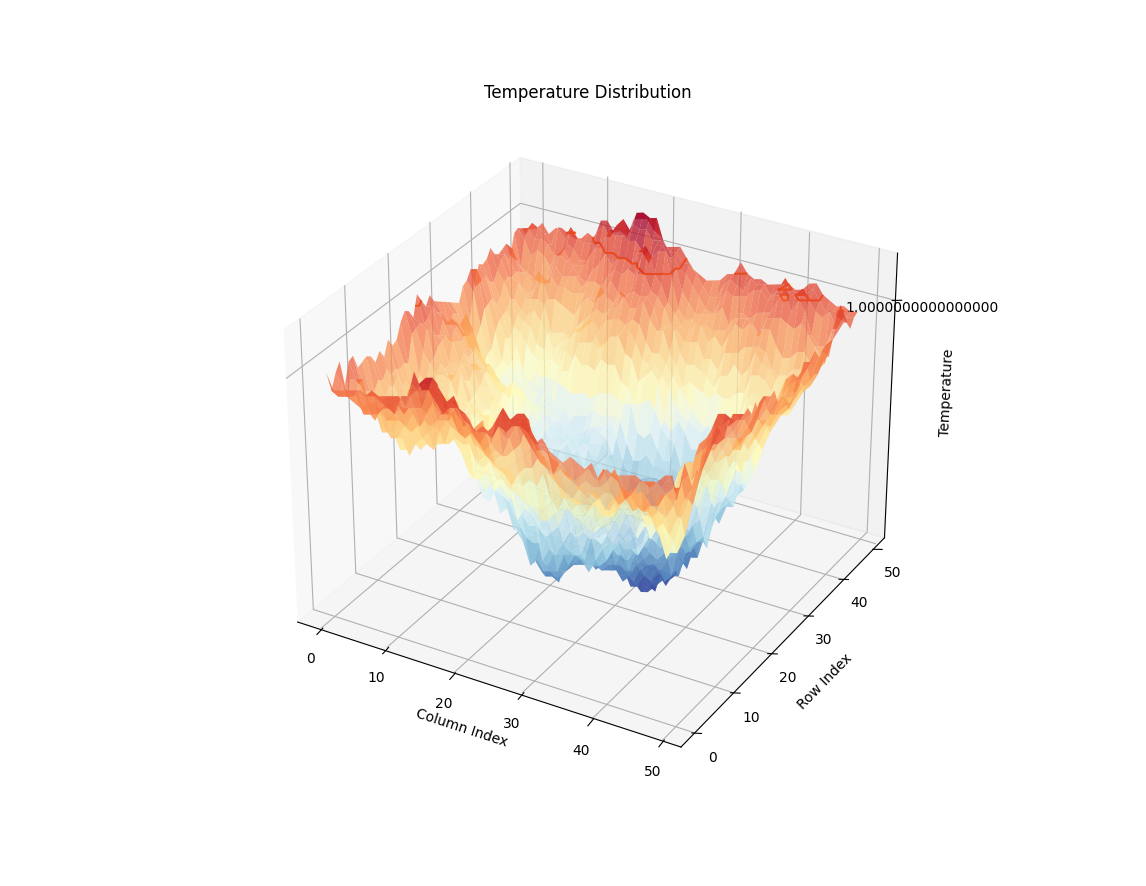
\includegraphics[width=\linewidth]{figures/Figure_8.png}
    \caption{3D Plot}
  \end{subfigure}
  \caption{Boundaries $T_{\text{left}}=1, T_{\text{up}}=1, T_{\text{right}}=1, T_{\text{down}}=1$ (edge case)}
\end{figure}

\begin{multicols}{2}
  
\section{Conclusion}
In this study, we explored the application of linear algebra techniques to
solve the numerical problem of determining equilibrium temperature
distributions within a plate. The motivation for this research arises from the
heat equation and its steady-state form, Laplace's equation, which describes
the spatial distribution of temperature in a system at thermal equilibrium.

We formulated the problem as a system of linear equations, with the unknown
temperatures at each lattice point represented by a vector. By leveraging the
mean-value property of solutions to Laplace's equation, we derived a system of
equations that could be expressed in matrix form. Two methods were employed for
solving this system: the inverse matrix method and Jacobi iterations.

The results obtained through these numerical methods provided insights into the
temperature distribution within the plate based solely on the boundary
conditions. Visualization of the equilibrium temperature distribution was
achieved through 2D and 3D plots, enhancing our understanding of the spatial
variation of temperatures.

The presented approach not only serves as a practical method for solving such
problems but also highlights the versatility of linear algebra in addressing
challenges in the field of thermodynamics. The ability to numerically determine
temperature distributions within a plate contributes to the broader
understanding of heat transfer phenomena and has potential applications in
various engineering and scientific domains.

In conclusion, this study demonstrates the effective use of linear algebra
techniques in solving real-world problems related to heat distribution. Future
work may involve extending this approach to more complex geometries or
incorporating additional physical factors into the model. Overall, the methods
presented here provide a valuable framework for tackling problems in heat
conduction and equilibrium temperature distributions.
\end{multicols}

\printbibliography[title=References, heading=bibnumbered]

% Appendix
\appendix
\section{Complementary Resources}
\begin{itemize}
  \item \href{https://github.com/salastro/etd-la}{Code Repository}
  \item \href{https://youtu.be/Zn6hnecikcc}{Iterations Video (Boundaries $T_{\text{left}}=2,
    T_{\text{up}}=2, T_{\text{right}}=1, T_{\text{down}}=0$)}
\end{itemize}

\end{document}
